\documentclass[a4paper]{article}
\usepackage[warn]{mathtext} %для поддержки кириллицы в формулах
\usepackage{amsmath} %основной пакет для формул
\usepackage[utf8x]{inputenc}
\usepackage[T1,T2A]{fontenc}
\usepackage[russian]{babel}
\usepackage{hyperref}
\usepackage{indentfirst}
\usepackage{listings}
\usepackage{color}
\usepackage{xcolor}
\usepackage{here}
\usepackage{array}
\usepackage{multirow}
\usepackage{graphicx}

\definecolor{linkcolor}{HTML}{000000} % цвет ссылок 000000 = чёрный
\definecolor{urlcolor}{HTML}{0000FF} % цвет гиперссылок 0000FF = синий
 
\hypersetup{pdfstartview=FitH, pagecolor=black, linkcolor=linkcolor,urlcolor=urlcolor, colorlinks=true}
\usepackage{caption}

\renewcommand{\lstlistingname}{Программа} % заголовок листингов кода

\usepackage{listings}
\lstset{ %
extendedchars=\true,
keepspaces=true,
language=c++,					% choose the language of the code
basicstyle=\footnotesize,		% the size of the fonts that are used for the code
numbers=left,					% where to put the line-numbers
numberstyle=\footnotesize,		% the size of the fonts that are used for the line-numbers
stepnumber=1,					% the step between two line-numbers. If it is 1 each line will be numbered
numbersep=5pt,					% how far the line-numbers are from the code
backgroundcolor=\color{white},	% choose the background color. You must add \usepackage{color}
showspaces=false				% show spaces adding particular underscores
showstringspaces=false,			% underline spaces within strings
showtabs=false,					% show tabs within strings adding particular underscores
frame=single,           		% adds a frame around the code
tabsize=2,						% sets default tabsize to 2 spaces
captionpos=b,					% sets the caption-position to bottom
breaklines=true,				% sets automatic line breaking
breakatwhitespace=false,		% sets if automatic breaks should only happen at whitespace
escapeinside={\%*}{*)},			% if you want to add a comment within your code
postbreak=\raisebox{0ex}[0ex][0ex]{\ensuremath{\color{red}\hookrightarrow\space}}
}

\usepackage[left=2cm,right=2cm,
top=2cm,bottom=2cm,bindingoffset=0cm]{geometry}

\newcommand{\RomanNumeralCaps}[1]
    {\MakeUppercase{\romannumeral #1}}


\begin{document}	% начало документа

\begin{titlepage}	% начало титульной страницы

	\begin{center}		% выравнивание по центру

		\large Санкт-Петербургский политехнический университет Петра Великого\\
		\large Институт компьютерных наук и технологий \\
		\large Кафедра компьютерных систем и программных технологий\\[2cm]
		% название института, затем отступ 6см
		
		
\includegraphics[scale=0.7]{pics/spbpu.jpg}\\[2cm]		
		
		\huge Курсовой проект по программированию\\
		\large Покер <<Техасский Холдем>>\\[8cm]
	\end{center}


	\begin{flushright} % выравнивание по правому краю
		\begin{minipage}{0.25\textwidth} % врезка в половину ширины текста
			\begin{flushleft} % выровнять её содержимое по левому краю

				\large\textbf{Работу выполнил:}\\
				\large Ламтев ~А.Ю.\\
				\large {Группа:} 13501/4\\
				
				\large \textbf{Преподаватель:}\\
				\large Вылегжанина ~К.Д.

			\end{flushleft}
		\end{minipage}
	\end{flushright}
	
	\vfill % заполнить всё доступное ниже пространство

	\begin{center}
	\large Санкт-Петербург\\
	\large \the\year % вывести дату
	\end{center} % закончить выравнивание по центру

\thispagestyle{empty} % не нумеровать страницу
\end{titlepage} % конец титульной страницы

\vfill % заполнить всё доступное ниже пространство



% Содержание
\hypertarget{toc}
\tableofcontents
\newpage

%TODO

\section*{Глава 1. Покер <<Техасский Холдем>>}
\addcontentsline{toc}{section}{Глава 1. Покер <<Техасский Холдем>>}

%Глава -- Описание предметной области (должно называться типа "Японская игра Сеги", "Эмулятор звездной системы", "Модель хищник-жертва" и %т. п.). Там размещаем то, что есть в ваших репозиториях в README.md, кроме диаграммы компонентов.\\


\subsection*{Задание}
\addcontentsline{toc}{subsection}{Задание}
	Используя код, написанный в прошлом семестре, разработать веб-сервер для игры покер, и разработать клиентское приложение под android.
 
\subsection*{Концепция}
\addcontentsline{toc}{subsection}{Концепция}

  Готовый программный продукт включает в себя веб-сервер, способный поддерживать игру нескольких человек (больше 1) против "компьютера" и против друг друга, а так же андроид-клиента, с которого можно осуществлять игру.

Расширением функциональности может быть поддержка высокой нагрузки на сервер.

\subsection*{Минимально работоспособный продукт (Minimum Viable Product - MVP)}
\addcontentsline{toc}{subsection}{Минимально работоспособный продукт (Minimum Viable Product - MVP)}

 Веб-сервер, поддерживающий игру человека против "компьютера", и андроид-клиент, с которого человек подключается к серверу и на котором осуществляет управление игрой.



\section*{Глава 2. Проектирование веб-сервера и android-клиента.}
\addcontentsline{toc}{section}{Глава 2. Проектирование приложения, реализующего игру Покер <<Техасский Холдем>>}

%Глава -- Проектирование ("Проектирование приложения, реализующего эмулятор звездной системы/японскую игру сеги/модель хищник-жертва". %Здесь описываете архитектуру приложения -- сколько каких подпроектов (какие библиотеки, приложения, тесты), диаграмма компонентов, %описание выделенных интерфейсов (API) человеческим языком, дополнительных библиотек (если использовали), версии языка, кьюти, %компилятора. Описать структуру файлов, если какие-то создаются в процессе работы приложения.\\

\subsection*{Веб-сервер}
\addcontentsline{toc}{section}{Веб-сервер}

В ходе проектрирования веб-сервера, было принято решение сделать его с REST API.

\begin{figure}[H]
	\begin{center}
		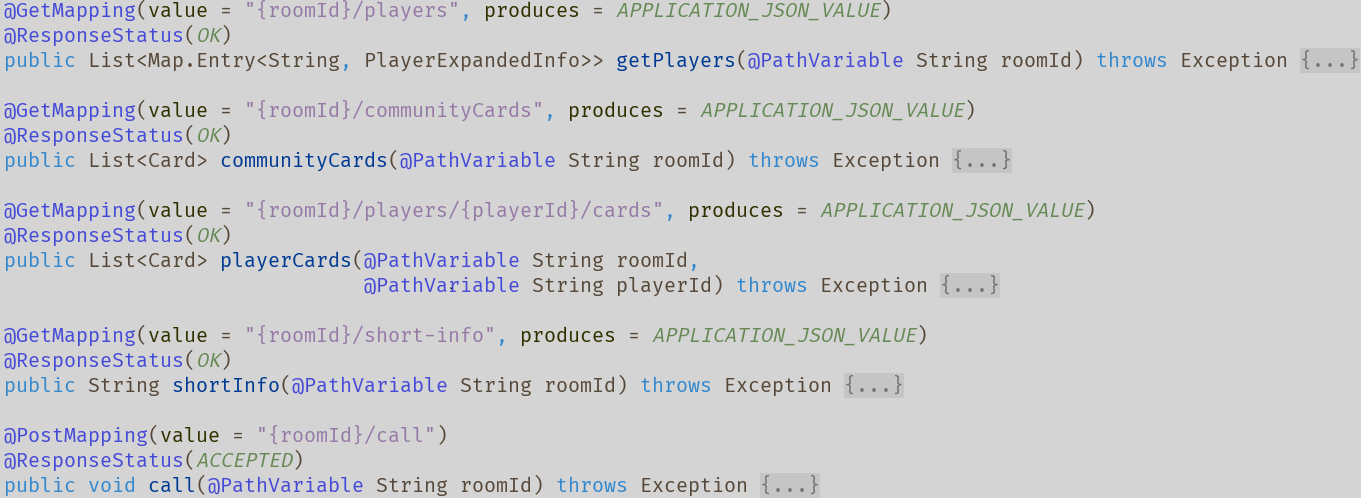
\includegraphics[scale=0.6]{pics/rest1}
	    \caption{Rest api} 
		\label{pic:rest:1}
	\end{center}
\end{figure}

~

\begin{figure}[H]
	\begin{center}
		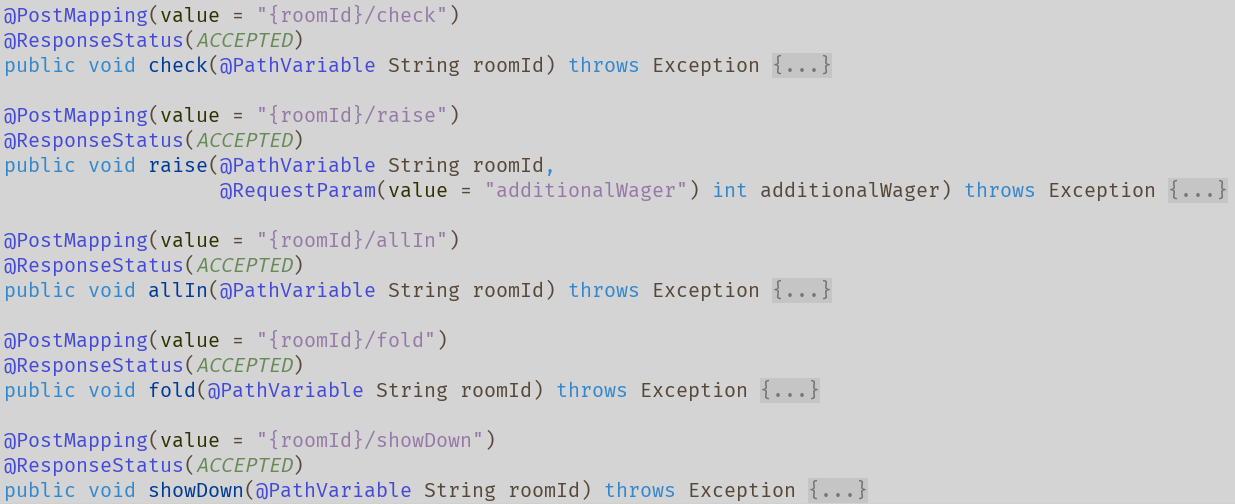
\includegraphics[scale=0.6]{pics/rest2}
	    \caption{Rest api} 
		\label{pic:rest:2}
	\end{center}
\end{figure}

~

\begin{figure}[H]
	\begin{center}
		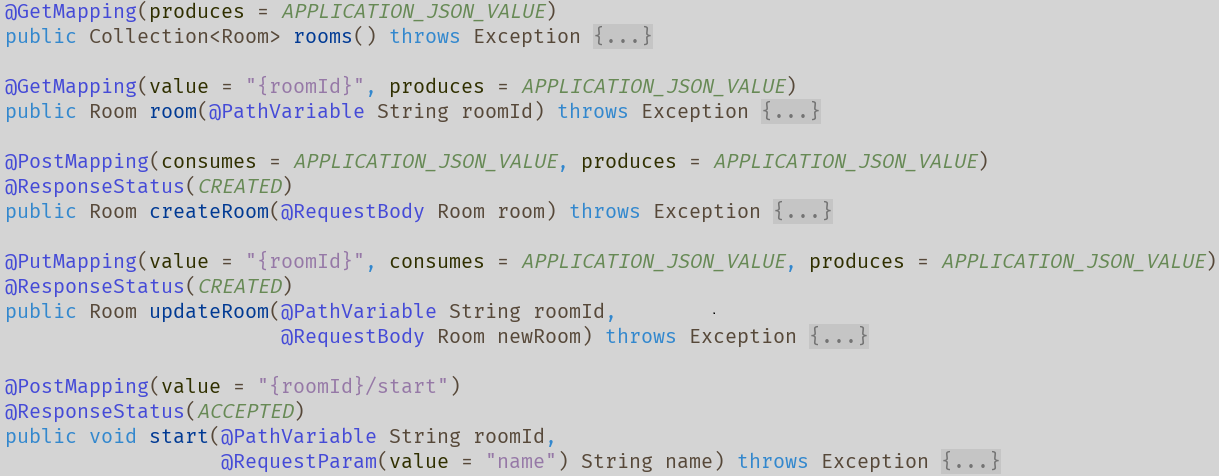
\includegraphics[scale=0.6]{pics/rest3}
	    \caption{Rest api} 
		\label{pic:rest:3}
	\end{center}
\end{figure}

\subsection*{Андроид-клиент}
\addcontentsline{toc}{section}{Андроид-клиент}

Андроид-клиент было принято решение делать в соответствии с Materail Design.

\subsection*{Вывод}
\addcontentsline{toc}{subsection}{Вывод}

В ходе проектирования было принято решение сделать restful веб-сервер и  material design андроид-клиент.

\section*{Глава 3. Реализация игры Покер <<Техасский Холдем>>}
\addcontentsline{toc}{section}{Глава 3. Реализация игры Покер <<Техасский Холдем>>}

%Глава -- Реализация ("Реализация японской игры сеги/модели хищник-жертва"). Здесь описываете среду разработки (версии всех использованых %ос, компиляторов, сред, утилит (qt creator, doxygen, прочее)), очень поверхностно описываете, какие основные классы выделили в каждом из %проектов, если какие-то интересные паттерны или алгоритмы -- тоже. Можно тут рассказать, сколько строк кода. Приводите скрины основных %%экранов пользовательского интерфейса, но чтоб не только картинки, но еще и слова, описывающие то, что видно на картинке. К картинкам не %забывайте делать подписи.

\subsection*{Среда разработки}
\addcontentsline{toc}{subsection}{Среда разработки}

\noindent\textbf{Операционная система:} Windows 10.0.10586\\
\textbf{Интегрированная среда разработки:} JetBrains IntelliJ IDEA 2016.3.3 -- 2017.1.3\\
\textbf{Уровень языка Java:} java 8 standart edition\\
\textbf{Компилятор:} jdk 1.8.0\_131\\
\textbf{Фреймворк для веб-сервера:} Spring Boot 1.5.3\\
\textbf{Android SDK:} 25\\
\textbf{Система автоматизации сборки:} Gradle 3.3 -- 3.5\\
\textbf{Система контроля версий:} Git 2.9.2\\

В ходе разработки приложения пришлось внести изменения в бизнес-логику покера, которая была разработана в предыдущем семестре.

\subsection*{Веб-сервер}
\addcontentsline{toc}{subsection}{Веб-сервер}

Веб-сервер разработан с использованием фреймворка Spring Boot и java 8.

\begin{figure}[H]
	\begin{center}
		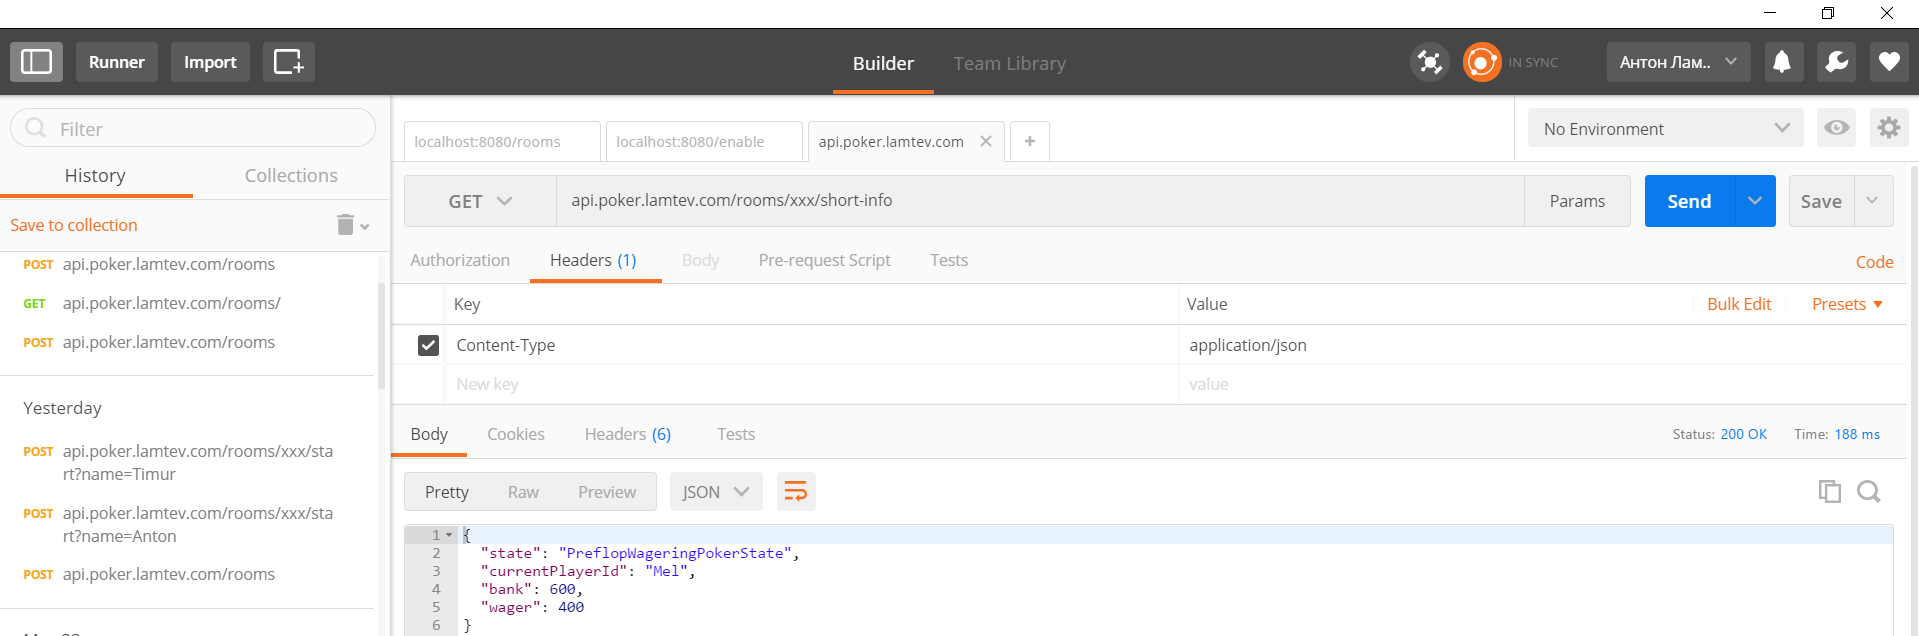
\includegraphics[scale=0.35]{pics/impl_rest}
	    \caption{Подключение к серверу по rest api через Postman} 
		\label{pic:gui:6}
	\end{center}
\end{figure}

Веб-приложение было развернуто на \textbf{heroku}\footnote{http://api.poker.lamtev.com}. 

\subsection*{Андроид-клиент}
\addcontentsline{toc}{subsection}{Андроид-клиент}

Андроид-клиент разработан c android sdk 25. Минимальный поддерживаемый уровень android-api -- 16. Среди компонентов разметки используются NavigationDrawer, FloatingActionBar, CardView, ConstraintLayout, LinearLayout, Textview, EditText, Button.

\begin{figure}[H]
	\begin{center}
		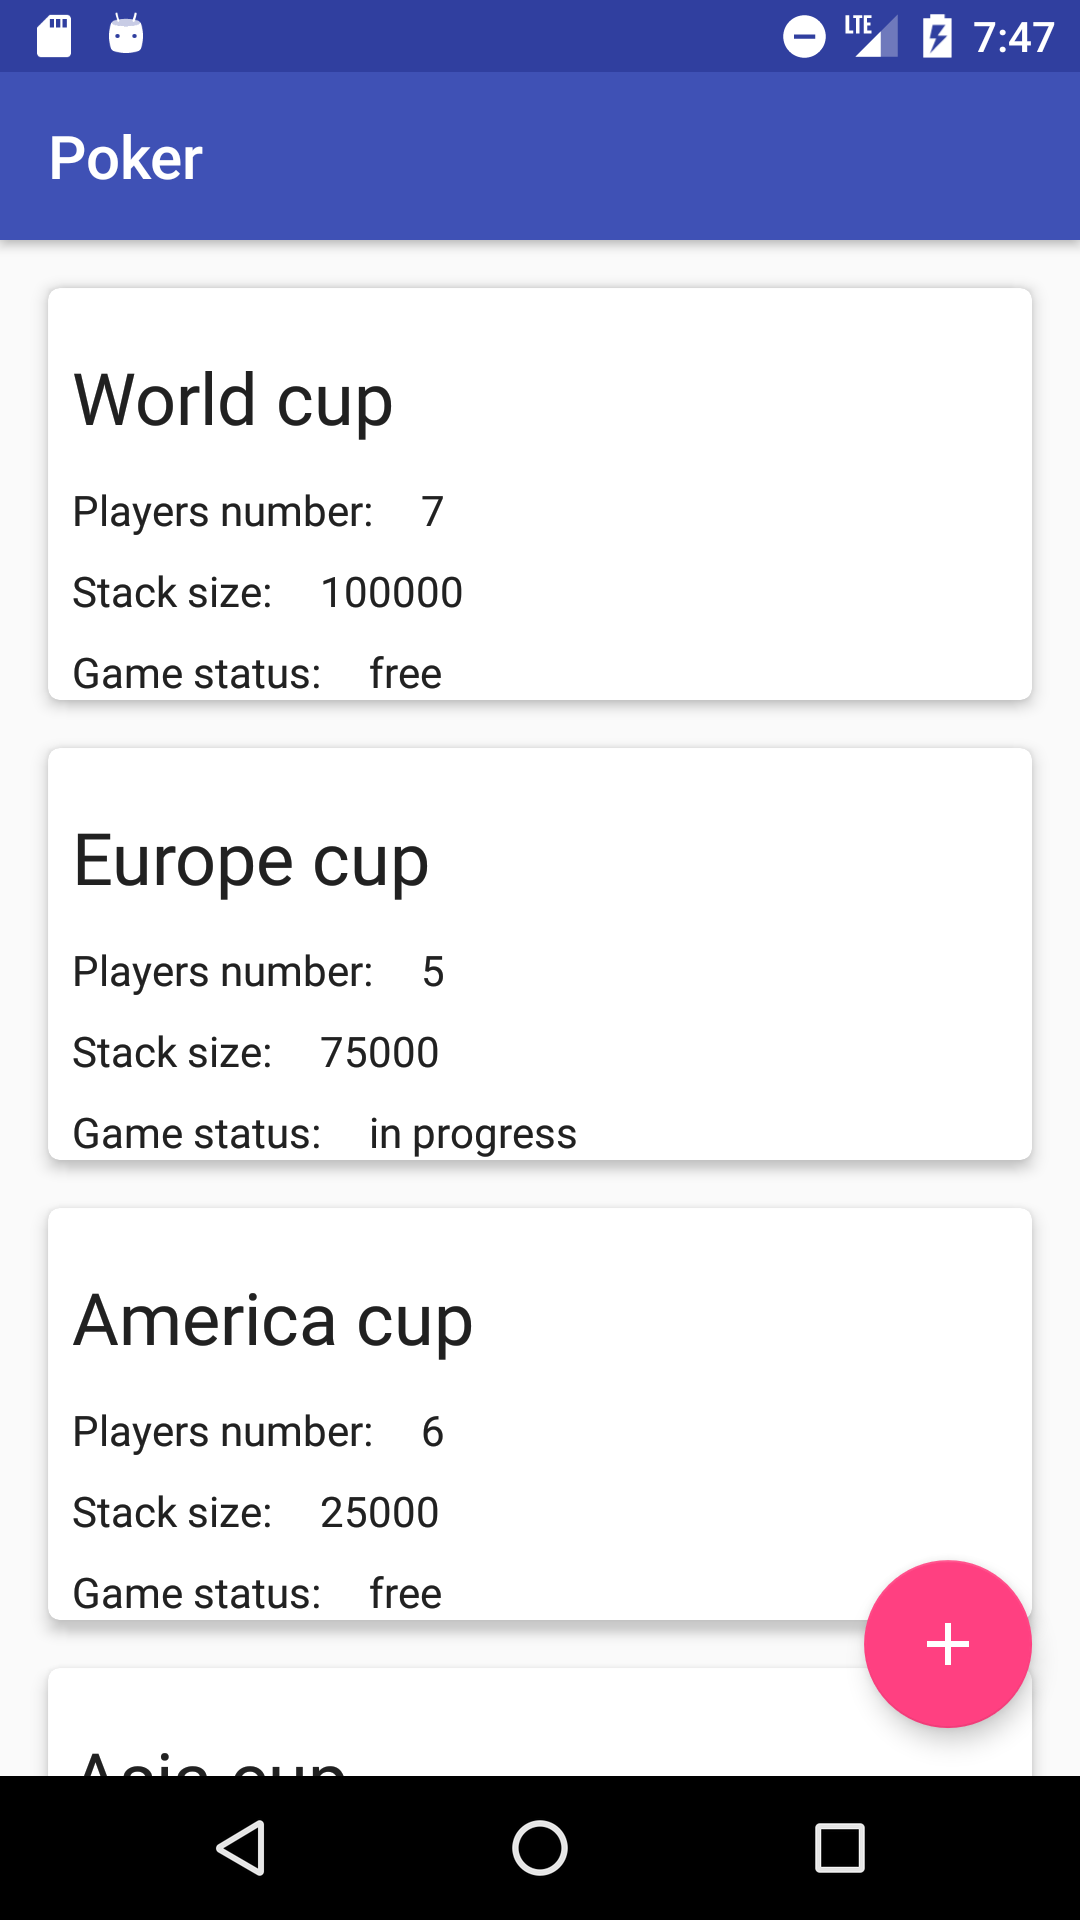
\includegraphics[scale=0.15]{pics/andr1}
	    \caption{Андроид-клиент, главный экран} 
		\label{pic:andr:1}
	\end{center}
\end{figure}

\begin{figure}[H]
	\begin{center}
		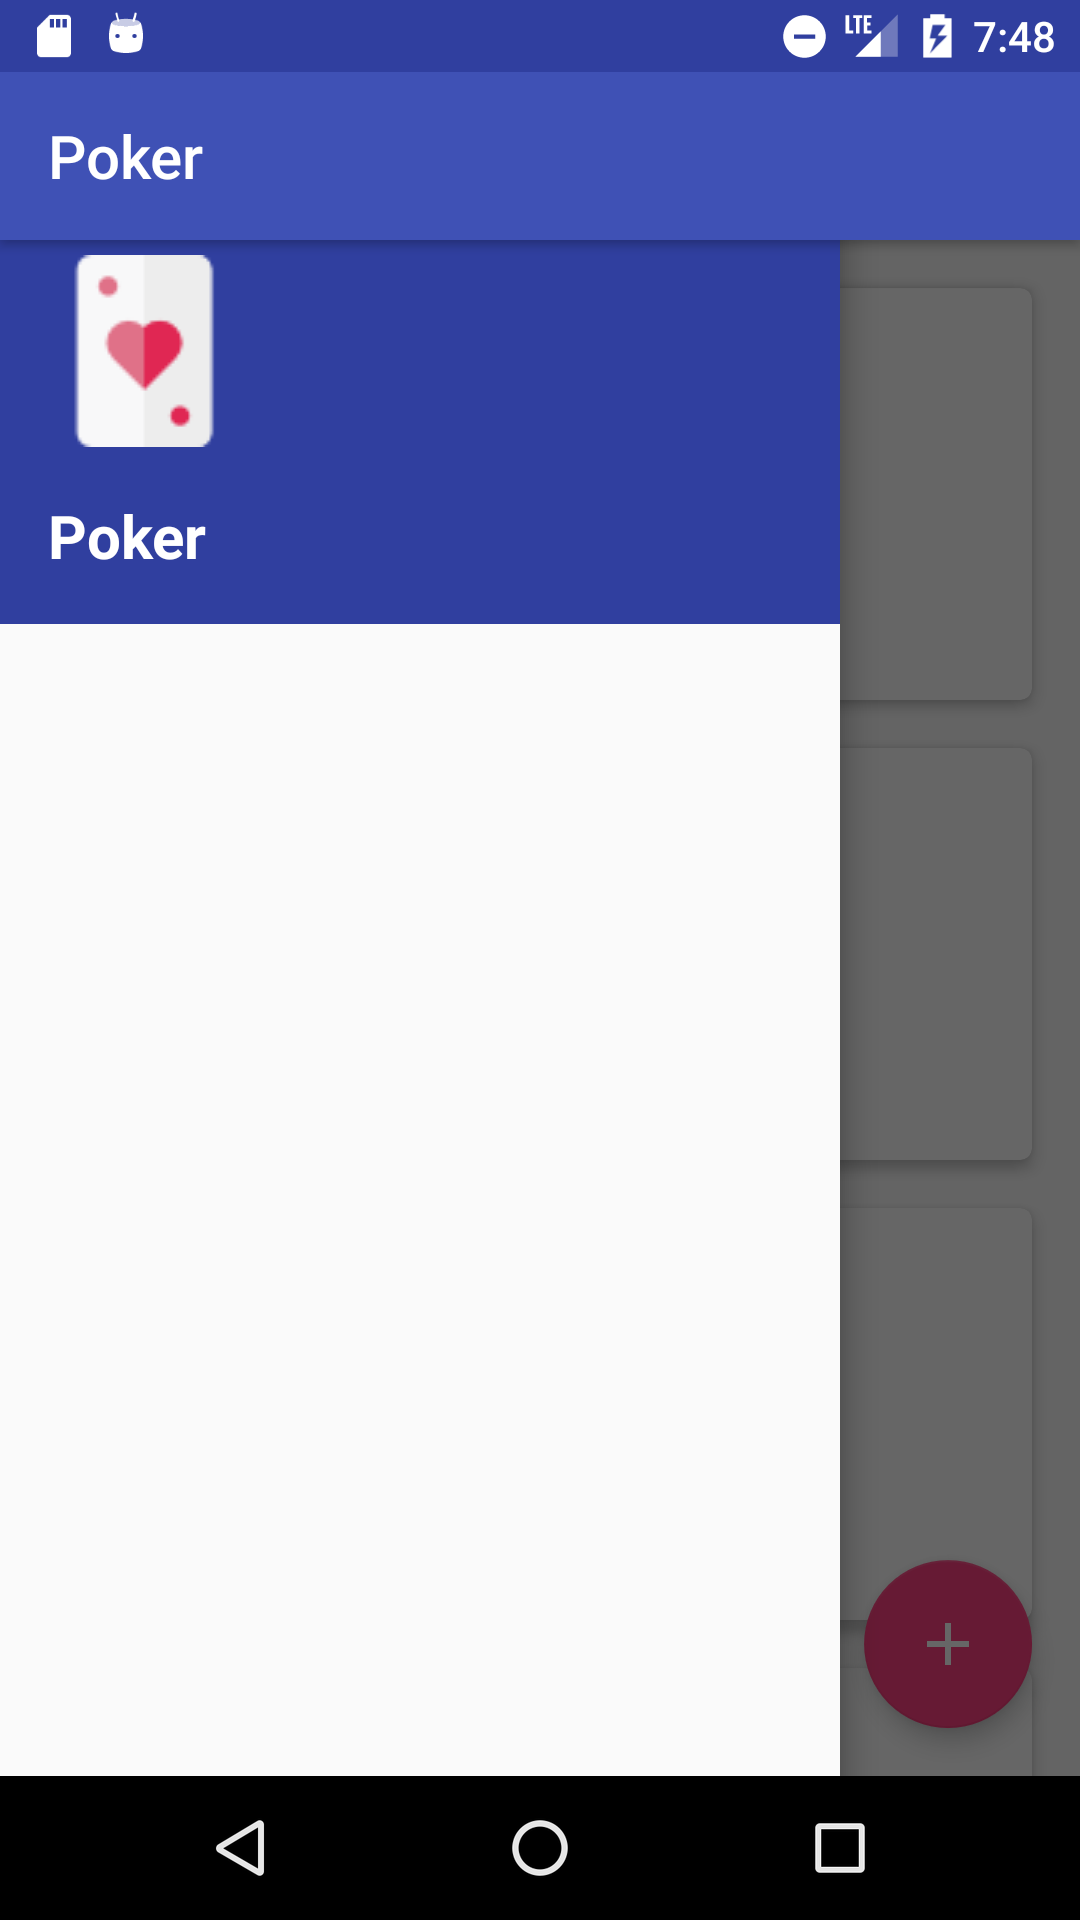
\includegraphics[scale=0.15]{pics/andr2}
	    \caption{Андроид-клиент, боковое меню} 
		\label{pic:andr:2}
	\end{center}
\end{figure}

\begin{figure}[H]
	\begin{center}
		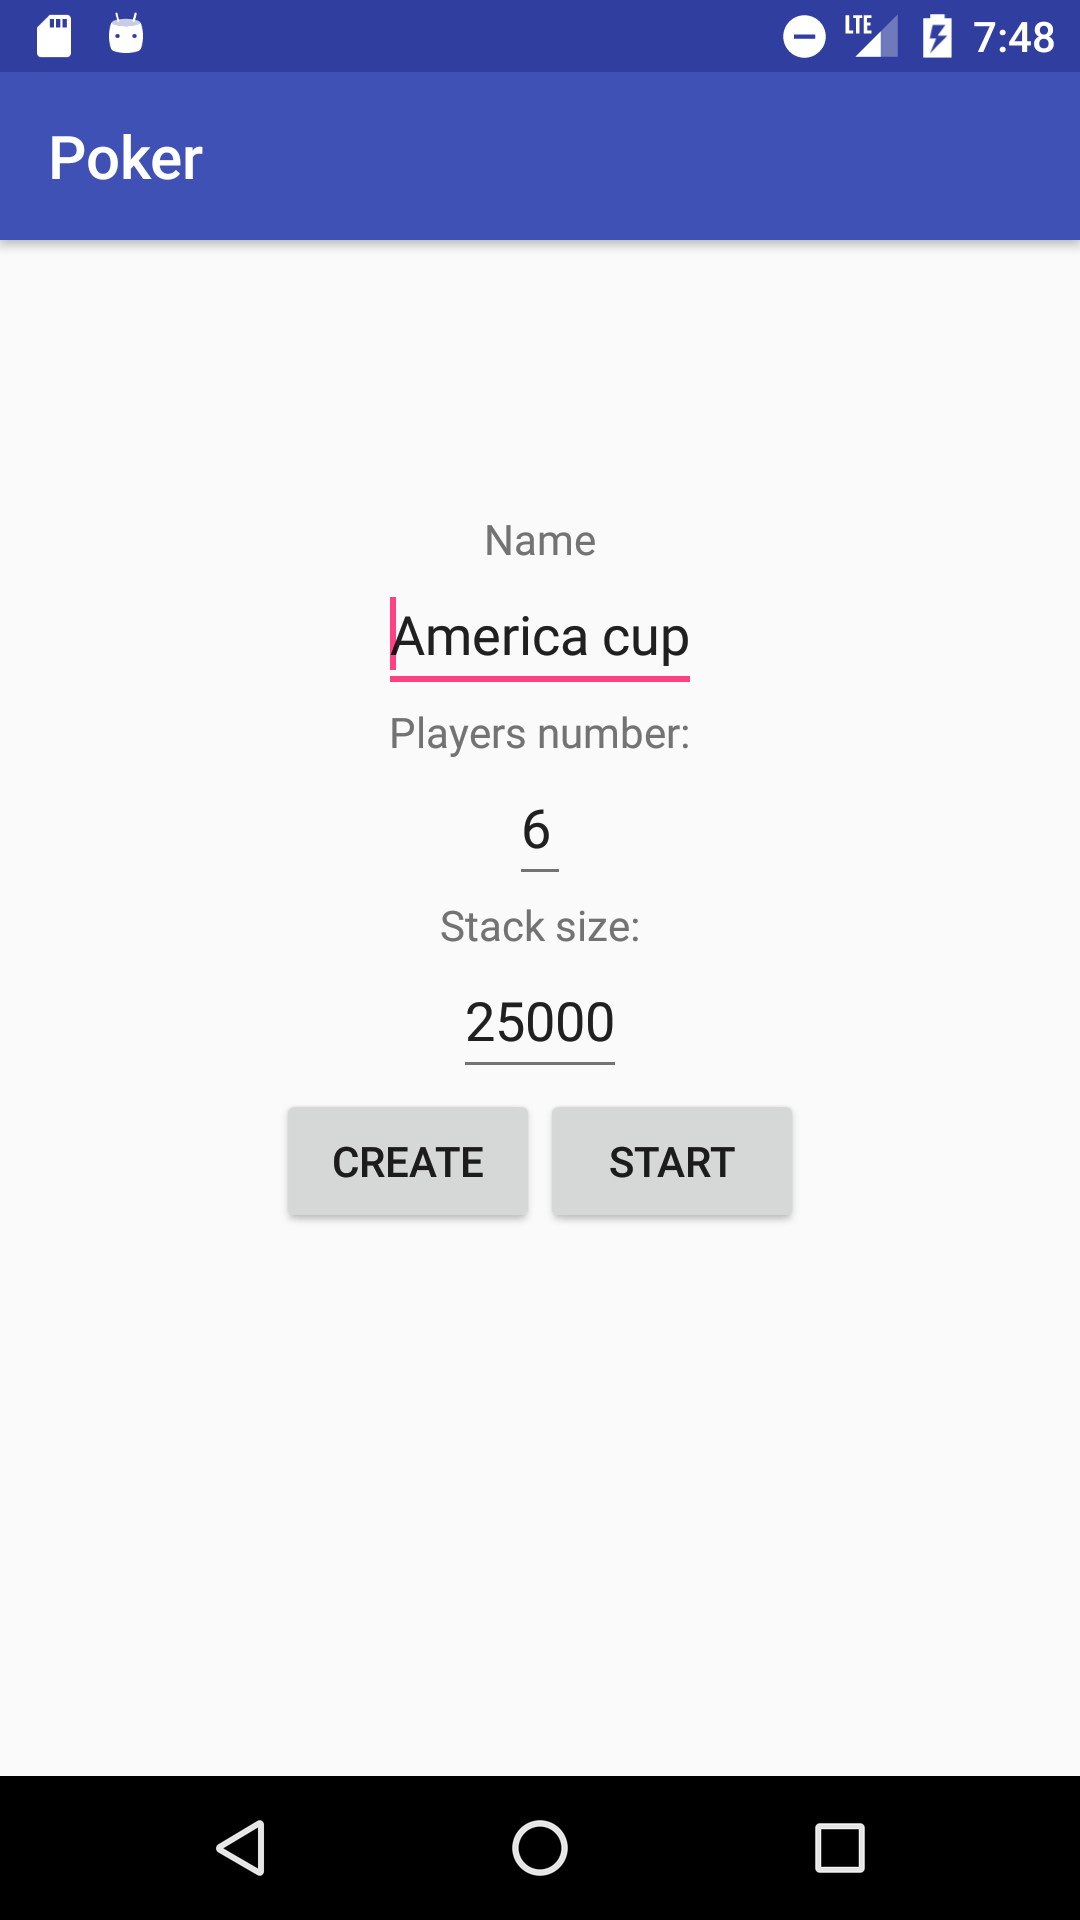
\includegraphics[scale=0.15]{pics/andr3}
	    \caption{Андроид-клиент, редактирование комнаты} 
		\label{pic:andr:3}
	\end{center}
\end{figure}



\subsection*{Вывод}
\addcontentsline{toc}{subsection}{Вывод}

В ходе разработки приложения автор получил большой опыт в в разработке resful веб-сервера и в разработке приложений для андроид. Клиентское приложение на данный момент способно лишь на чтение данных.

\section*{Глава 4. Процесс обеспечения качества и тестирование}
\addcontentsline{toc}{section}{Глава 4. Процесс обеспечения качества и тестирование}

%Глава -- "Процесс обеспечения качества и тестирование". Здесь описываете процесс разработки -- количество ревью (и примерное количество %замечаний), количество демонстраций (с указанием конкретных замечаний и комментариями по ним), список использованных утилит (cppcheck, %valgrind, gcov и т.д, кто пользовался jenkins -- про него тоже) с комментариями как и когда они помогали. Рассказать про автоматические %тесты (модульные, функциональные), про тестовые сценарии, которые они покрывают, процент покрытия. Рассказать про тестовые сценарии для %ручных тестов.

Разработка велась в цикле непрерывной интеграции (continuous integration - ci). Кроме того, она сопровождалась ручным и автоматическим(модульным и функциональным) тестированием, статическим анализом кода, просмотрами кода (code review).

\subsection*{Тестирование}
\addcontentsline{toc}{subsection}{Тестирование}

\subsubsection*{Автоматическое тестирование}
\addcontentsline{toc}{subsubsection}{Автоматическое тестирование}

Частично разработка велась согласно подходу TDD (Test-Driven Development), когда сначала сразу после проектирования интерфейса класса пишутся модульные тесты, а затем реализуется функциональность класса. 

Для веб-сервера написаны интеграционные тесты (SpringBootTest), в ходе которых проверяется правильность обработки сервером запросов.

Для автоматического тестирования использовался фреймворк JUnit 4.12.

Для удобного отображения результатов подсчета покрытия тестами кода использовался сервис Codecov \footnote{https://codecov.io}
Процент покрытия 87 \%.

\subsection*{Статический анализ}
\addcontentsline{toc}{subsubsection}{Статический анализ}

Статический анализ проводился при помощи JetBrains IntelliJ IDEA inspections, find-bugs и android lint. Практически все найденные ими недочеты в коде были исправленны.

\subsection*{Непрерывная интеграция}
\addcontentsline{toc}{subsection}{Непрерывная интеграция}

Непрерывная интеграция осуществлялась с помощью платформы Travic-ci.\footnote{https://travis-ci.org}
	
В цикле ci внутри cобственных \textbf{docker} контейнеров \textbf{lamtev/java}\footnote{https://hub.docker.com/r/lamtev/java/} и \textbf{lamtev/android}\footnote{https://hub.docker.com/r/lamtev/android/} запускались автоматические тесты, код анализировался статическим анализатором, велся подсчёт строк (утилита cloc 1.60).

На рис. \ref{pic:travis:3} приведен снимок экрана, на котором показано, что проект около содержит 5000 строк кода на java

\begin{figure}[H]
	\begin{center}
		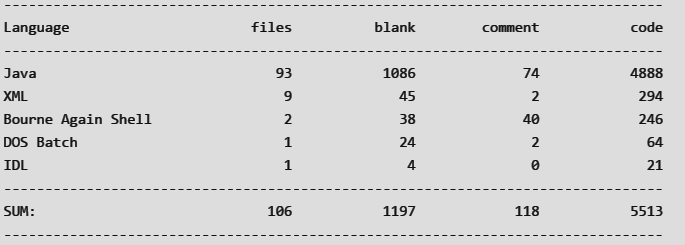
\includegraphics[scale=0.75]{pics/travis2.png}
	    \caption{Travis-ci: cloc} 
		\label{pic:travis:3}
	\end{center}
\end{figure}

\subsection*{Просмотр кода (Code Review)}
\addcontentsline{toc}{subsection}{Просмотр кода (Code Review)}

Автор в ходе разработки просил своих коллег: Дьячкова Вадима и Леженина Юрия посмотреть его код. После их советов и указаний на недочеты в коде, были внесены правки.

\subsection*{Вывод}
\addcontentsline{toc}{subsection}{Вывод}

В ходе процесса обеспечения качества и тестирования автор получил навык написания кода, который легко тестировать. Автор получил опыт от использования непрерывной интеграции. Был получен опыт улучшения качества кода после code review от коллег.

\section*{Глава 5. Выводы}
\addcontentsline{toc}{section}{Глава 5. Выводы}

%своими словами, с душой, от чистого сердца рассказать, чему удалось научиться за семестр, что извлечь.
За семестр были получены первые навыки проектирования и разработки restful веб-сервера и андроид-приложения.

В итоге получилось разбработать минимально работоспособный продукт.

Автор продолжит разработку данного приложения в соответствии с концепцией.

\section*{Приложение. Листинги}

\lstinputlisting[
	label=code:rest,
	caption={Rest.java},% для печати символ '_' требует выходной символ '\'
]{../../webserver/src/main/java/com/lamtev/poker/webserver/Rest.java}
\parindent=1cm % командна \lstinputlisting сбивает параментры отступа

\lstinputlisting[
	label=code:GameAPI,
	caption={GameAPI.java},% для печати символ '_' требует выходной символ '\'
]{../../webserver/src/main/java/com/lamtev/poker/webserver/GameAPI.java}
\parindent=1cm % командна \lstinputlisting сбивает параментры отступа

\lstinputlisting[
	label=code:Game,
	caption={Game.java},% для печати символ '_' требует выходной символ '\'
]{../../webserver/src/main/java/com/lamtev/poker/webserver/Game.java}
\parindent=1cm % командна \lstinputlisting сбивает параментры отступа

\lstinputlisting[
	label=code:Room,
	caption={Room.java},% для печати символ '_' требует выходной символ '\'
]{../../webserver/src/main/java/com/lamtev/poker/webserver/Room.java}
\parindent=1cm % командна \lstinputlisting сбивает параментры отступа

\lstinputlisting[
	label=code:Room,
	caption={Util.java},% для печати символ '_' требует выходной символ '\'
]{../../webserver/src/main/java/com/lamtev/poker/webserver/Util.java}
\parindent=1cm % командна \lstinputlisting сбивает параментры отступа

\lstinputlisting[
	label=code:Room,
	caption={AbstractController.java},% для печати символ '_' требует выходной символ '\'
]{../../webserver/src/main/java/com/lamtev/poker/webserver/controllers/AbstractController.java}
\parindent=1cm % командна \lstinputlisting сбивает параментры отступа

\lstinputlisting[
	label=code:RoomsC,
	caption={RoomsController.java},% для печати символ '_' требует выходной символ '\'
]{../../webserver/src/main/java/com/lamtev/poker/webserver/controllers/RoomsController.java}
\parindent=1cm % командна \lstinputlisting сбивает параментры отступа

\lstinputlisting[
	label=code:Room,
	caption={GameController.java},% для печати символ '_' требует выходной символ '\'
]{../../webserver/src/main/java/com/lamtev/poker/webserver/controllers/GameController.java}
\parindent=1cm % командна \lstinputlisting сбивает параментры отступа

\lstinputlisting[
	label=code:Room,
	caption={NoCardsException.java},% для печати символ '_' требует выходной символ '\'
]{../../webserver/src/main/java/com/lamtev/poker/webserver/controllers/exceptions/NoCardsException.java}
\parindent=1cm % командна \lstinputlisting сбивает параментры отступа

\lstinputlisting[
	label=code:Room,
	caption={RequestBodyHasUnsuitableFormatException.java},% для печати символ '_' требует выходной символ '\'
]{../../webserver/src/main/java/com/lamtev/poker/webserver/controllers/exceptions/RequestBodyHasUnsuitableFormatException.java}
\parindent=1cm % командна \lstinputlisting сбивает параментры отступа

\lstinputlisting[
	label=code:Room,
	caption={ResourceAlreadyExistsException.java},% для печати символ '_' требует выходной символ '\'
]{../../webserver/src/main/java/com/lamtev/poker/webserver/controllers/exceptions/ResourceAlreadyExistsException.java}
\parindent=1cm % командна \lstinputlisting сбивает параментры отступа

\lstinputlisting[
	label=code:Room,
	caption={ResourceNotFoundException.java},% для печати символ '_' требует выходной символ '\'
]{../../webserver/src/main/java/com/lamtev/poker/webserver/controllers/exceptions/ResourceNotFoundException.java}
\parindent=1cm % командна \lstinputlisting сбивает параментры отступа

\lstinputlisting[
	label=code:Room,
	caption={RoomStatusException.java},% для печати символ '_' требует выходной символ '\'
]{../../webserver/src/main/java/com/lamtev/poker/webserver/controllers/exceptions/RoomStatusException.java}
\parindent=1cm % командна \lstinputlisting сбивает параментры отступа


\lstinputlisting[
	label=code:Room,
	caption={AbstractExceptionHandler.java},% для печати символ '_' требует выходной символ '\'
]{../../webserver/src/main/java/com/lamtev/poker/webserver/exception_handlers/AbstractExceptionHandler.java}
\parindent=1cm % командна \lstinputlisting сбивает параментры отступа

\lstinputlisting[
	label=code:Room,
	caption={GameControllerExceptionHandler.java},% для печати символ '_' требует выходной символ '\'
]{../../webserver/src/main/java/com/lamtev/poker/webserver/exception_handlers/GameControllerExceptionHandler.java}
\parindent=1cm % командна \lstinputlisting сбивает параментры отступа

\lstinputlisting[
	label=code:Room,
	caption={RoomsControllerExceptionHandler.java},% для печати символ '_' требует выходной символ '\'
]{../../webserver/src/main/java/com/lamtev/poker/webserver/exception_handlers/RoomsControllerExceptionHandler.java}
\parindent=1cm % командна \lstinputlisting сбивает параментры отступа

\lstinputlisting[
	label=code:Room,
	caption={ResponseMessage.java},% для печати символ '_' требует выходной символ '\'
]{../../webserver/src/main/java/com/lamtev/poker/webserver/exception_handlers/ResponseMessage.java}
\parindent=1cm % командна \lstinputlisting сбивает параментры отступа

\lstinputlisting[
	label=code:Room,
	caption={RoomsActivity.java},% для печати символ '_' требует выходной символ '\'
]{../../android/app/src/main/java/com/lamtev/poker/android/RoomsActivity.java}
\parindent=1cm % командна \lstinputlisting сбивает параментры отступа

\lstinputlisting[
	label=code:Room,
	caption={RoomActivity.java},% для печати символ '_' требует выходной символ '\'
]{../../android/app/src/main/java/com/lamtev/poker/android/RoomActivity.java}
\parindent=1cm % командна \lstinputlisting сбивает параментры отступа

\lstinputlisting[
	label=code:Room,
	caption={RoomListFragment.java},% для печати символ '_' требует выходной символ '\'
]{../../android/app/src/main/java/com/lamtev/poker/android/RoomListFragment.java}
\parindent=1cm % командна \lstinputlisting сбивает параментры отступа

\lstinputlisting[
	label=code:Room,
	caption={RoomInfo.java},% для печати символ '_' требует выходной символ '\'
]{../../android/app/src/main/java/com/lamtev/poker/android/RoomInfo.java}
\parindent=1cm % командна \lstinputlisting сбивает параментры отступа

\lstinputlisting[
	label=code:Room,
	caption={activity\_rooms.xml},% для печати символ '_' требует выходной символ '\'
]{../../android/app/src/main/res/layout/activity_rooms.xml}
\parindent=1cm % командна \lstinputlisting сбивает параментры отступа

\lstinputlisting[
	label=code:Room,
	caption={activity\_room.xml},% для печати символ '_' требует выходной символ '\'
]{../../android/app/src/main/res/layout/activity_room.xml}
\parindent=1cm % командна \lstinputlisting сбивает параментры отступа

\lstinputlisting[
	label=code:Room,
	caption={fragment\_room\_card\_list.xml},% для печати символ '_' требует выходной символ '\'
]{../../android/app/src/main/res/layout/fragment_room_card_list.xml}
\parindent=1cm % командна \lstinputlisting сбивает параментры отступа

\lstinputlisting[
	label=code:Room,
	caption={navigation.xml},% для печати символ '_' требует выходной символ '\'
]{../../android/app/src/main/res/layout/navigation.xml}
\parindent=1cm % командна \lstinputlisting сбивает параментры отступа

\lstinputlisting[
	label=code:Room,
	caption={room\_card.xml},% для печати символ '_' требует выходной символ '\'
]{../../android/app/src/main/res/layout/room_card.xml}
\parindent=1cm % командна \lstinputlisting сбивает параментры отступа

\lstinputlisting[
	label=code:Room,
	caption={.travis.yml},% для печати символ '_' требует выходной символ '\'
]{../../.travis.yml}
\parindent=1cm % командна \lstinputlisting сбивает параментры отступа

\end{document}
